\subsubsection{LSA16} \cite{Ronchetti2016} contains images of 16 handshapes of the Argentinian Sign Language (LSA), each performed 5 times by 10 different subjects, for a total of 800 images of size 32x32. The subjects wore colored hand gloves and dark clothes on a white background. The dataset is balanced, with 50 images per class. There is only one hand in each image which are centered and isolated from the background.

\subsubsection{RWTH} \cite{koller16:deephand} is composed of a selection of  hand images of size 132x92 cropped from  videos of the sign language interpreters at the German public tv-station PHOENIX. There are a total of 45 different hand signs. The interpreters wore dark clothes in front of an artificial grey background. Many images posses significant movement blur,  others contain both hands of the interpreter and hands are not always perfectly centered.

The dataset is highly imbalanced with some classes having just 1 sample while others have as many as 529 samples. We removed classes that had less than 20 samples following \cite{quiroga2017study}, to guarantee a minimum amount of images per class for the networks to learn.

\subsubsection{CIARP} \cite{ciarp2018} contains 6000 images of size 38x38 adquired by a single color camera. The images were manually labeled and correspond to 10 classes of hand gestures. The hands are centered and were segmented from the background, which was replaced by black pixels. The small size of the images and low amount of classes give this dataset lower complexity compared to LSA16 and RWTH.  The  classes in the data set correspond to handshapes  not based on sign language, but are similar enough  that the comparison remains valid.

% TODO add reference to this figure in each datasets subsection
\begin{figure}
    \centering
    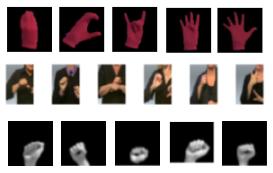
\includegraphics[width=0.8\textwidth]{datasets/samples.png}
    \caption{Sample images from the LSA16 (first row), RWTH-PHOENIX-Weather (second row) and CIARP (third row) datasets.}
    \label{fig:datasets}
\end{figure}